\documentclass{beamer}

\usetheme{Warsaw}
\beamertemplatenavigationsymbolsempty
\boldmath

\usepackage{graphicx}
\graphicspath{ {./images/} }

\title[Implementation of a Constructive Neural Network]{Design, Implementation and Testing of a Constructive Neural Network Algorithm}
\author[Andrea Orru]{\textbf{Andrea Orru} \small{(ID: 1473018)} \\ \small{Supervisor: Michael Spratling}}
\institute[King's College London]{Department of Informatics \\ King's College London}
\date{2014/2015}
\subject{MSc Intelligent Systems}

\begin{document}
	\frame{\titlepage}
	
	\begin{frame}
		\frametitle{Table of Contents}
		\tableofcontents
	\end{frame}
	
	\section{Introduction}
		\subsection{Problem and motivation}
			\begin{frame}
				\frametitle{Problem and motivation}
				\framesubtitle{Artificial Neural Networks and their topology}
				\begin{block}{Artificial Neural Networks}
					\emph{Artificial neural networks} are a powerful model in machine learning. In theory, an adequately large network is an \emph{universal approximator}.
				\end{block}
				\begin{figure}[h]
					\centering
					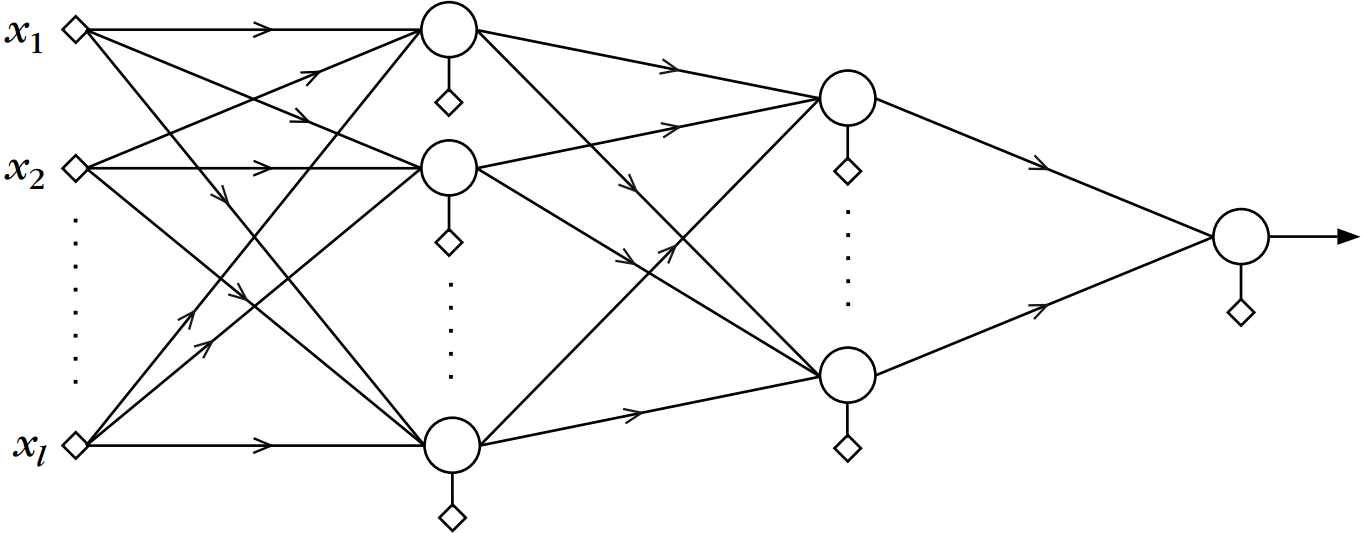
\includegraphics[width=0.65\textwidth]{multilayer}
				\end{figure}
				\begin{alertblock}{Topology}
					In practice, \textbf{too small} networks are unable to learn the problem, while \textbf{overly large} ones tend to \emph{overfit} the training data.
				\end{alertblock}
			\end{frame}
			\begin{frame}
				\frametitle{Problem and motivation}
				\framesubtitle{Choosing the topology}
				\begin{block}{Trial and error}
					The architecture of the network is often determined by \emph{trial and error} based on previous experience.
				\end{block}
				\begin{block}{Learning the topology}
					An interesting alternative is \textbf{discovering the topology} as part of the learning algorithm.
				\end{block}
				\begin{exampleblock}{Constructive Neural Network}
					Algorithms that starts from a minimal architecture and then add nodes, connections and layers are called \textbf{\emph{constructive}}.
				\end{exampleblock}
			\end{frame}
			\begin{frame}
				\frametitle{Problem and motivation}
				\framesubtitle{Problem definition}
				\begin{exampleblock}{The problem}
					In this project I developed a \textbf{constructive version} of the existing \emph{Divisive Input Modulation} algorithm.
				\end{exampleblock}
				\begin{block}{Why?}
					Small network are \textbf{faster} and \textbf{generalize} better.
				\end{block}
				\begin{block}{Divisive Input Modulation}
					DIM is an unsupervised training algorithm that has state-of-the-art performances in \textbf{image decomposition}.
				\end{block}
			\end{frame}
		
		\subsection{Background}
			\begin{frame}
				\frametitle{Image decomposition}
				\begin{block}{Image decomposition}
					Finding the \textbf{basic components} from which a set of images are formed, e.g. as a non-negative linear combination of features.
				\end{block}
				\begin{figure}[h]
					\centering
					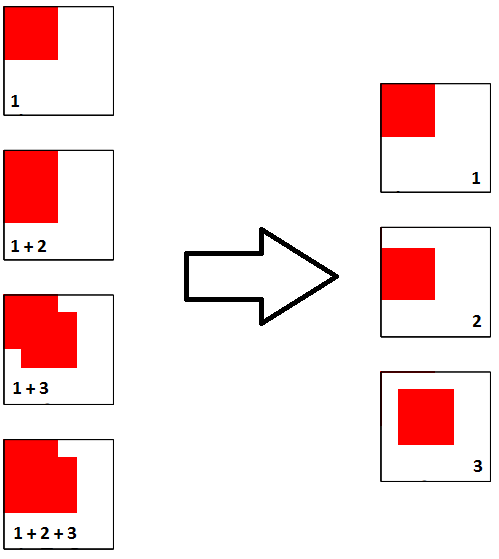
\includegraphics[width=0.45\textwidth]{decomposition}
				\end{figure}
			\end{frame}
			\begin{frame}
				\frametitle{Divisive Input Modulation}  
				\begin{columns}[c]
				    \column{0.2\textwidth}
						\begin{figure}[h]
							\centering
							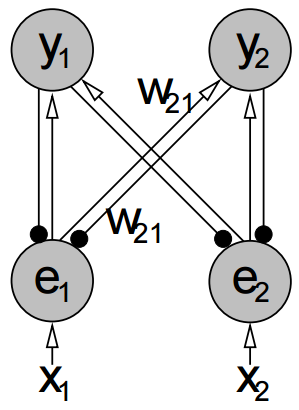
\includegraphics[width=\textwidth]{dim}
						\end{figure}
				    \column{0.8\textwidth}
					    \begin{block}{Inhibitory feedback}
					    	Activation from \emph{predictive} nodes $y_1 ... y_n$ is \textbf{fed back} to \emph{error-detecting} neurons $e_1 ... e_m$ which \emph{modulate} the inputs $x_1 ... x_m$, implementing \emph{competition}.
					    \end{block}
					    \begin{block}{Generative interpretation}
					    	\small{\begin{itemize}
					    		\item $e$: divisive measure of the error ($e_i = 1$ means perfect reconstruction);
					    		\item $W$: row $W_j$ of matrix contains weights to/from neuron $y_j$ and represents a \emph{basic component}.
					    		\item $y$: activation $y_j$ represents the importance of component $j$ in reconstruction of image $x_1 ... x_m$.
					    	\end{itemize}}
					    \end{block}
				\end{columns}
			\end{frame}
		
	\section{The constructive algorithm}
	
	\section{Conclusions}
		
\end{document}